\documentclass[10pt,twocolumn,letterpaper]{article}

\usepackage{cvpr}
\usepackage{times}
\usepackage{epsfig}
\usepackage{graphicx}
\usepackage{amsmath}
\usepackage{amssymb}

\usepackage{url}

% Include other packages here, before hyperref.

% If you comment hyperref and then uncomment it, you should delete
% egpaper.aux before re-running latex.  (Or just hit 'q' on the first latex
% run, let it finish, and you should be clear).
%\usepackage[pagebackref=true,breaklinks=true,letterpaper=true,colorlinks,bookmarks=false]{hyperref}

\cvprfinalcopy % *** Uncomment this line for the final submission

\def\cvprPaperID{****} % *** Enter the CVPR Paper ID here
\def\httilde{\mbox{\tt\raisebox{-.5ex}{\symbol{126}}}}

% Pages are numbered in submission mode, and unnumbered in camera-ready
\ifcvprfinal\pagestyle{empty}\fi
\begin{document}

%%%%%%%%% TITLE
\title{Image Classification Analysis with Bag of Word Model}

\author{Lorenzo Cioni\\
{\tt\small lore.cioni@gmail.com}
% For a paper whose authors are all at the same institution,
% omit the following lines up until the closing ``}''.
% Additional authors and addresses can be added with ``\and'',
% just like the second author.
% To save space, use either the email address or home page, not both
\and
Saverio Meucci\\
{\tt\small s.meucci91@gmail.com}
}

\maketitle
\thispagestyle{empty}

%%%%% ABSTRACT %%%%

\begin{abstract}

In this paper, we evaluated the performance of Nearest Neighbour and Support Vector Machine as images classifier, using Bag of Word model. Different metric functions and different kernel functions were taken into account. With regard to features quantization, we have focused our attention to soft-assignment and truncated soft-assignment, in comparison to hard-assignment.

\end{abstract}

%%%%% KEYWORDS %%%%

{\footnotesize \noindent\textbf{Keywords} - Bag of Words (BoW), SIFT, SVM, Nearest Neighbours, Hard-Soft Assignment}.


\section{Introduction}

In computer vision, the \emph{bag-of-words} model is one of the well established image classification methods. Not only comparing two image by matching each local features of the images is computationally intensive, but also different images have different number of local features. BoW model simplified this process by building a vocabulary of visual-words, called codebook. This way, an image descriptor is a histogram built by counting how many codewords are present in an image.

Given this model for image classification, we have compared how different classifiers performs.
We have studied the \emph{Nearest-Neighbor} (NN) classifier, comparing the results using both the Euclidean distance and the $\chi^2$ distance.

In addiction, we have examined the \emph{Support Vector Machine} (SVM) classifier, implementing different kernel functions; in particular, the linear kernel, the intersection kernel, the $\chi^2$ kernel, and the radial basis function kernel have been implemented.
In evaluating the performance of a classifiers, many parameters, that can vary the results, must be taken into account.
For instance, we have also compared the results on varying parameters like the density or sparseness of the key-points in each image, the dimension of the vocabulary and the dimension of the training set used to train the classifiers.

Another aspect that can influence the performance of a classifier, using the BoW model, is choosing between \emph{hard-assignment} and \emph{soft-assignment}. Briefly, with \emph{hard-assignment} each local features of an image is assigned to one codeword; with \emph{soft-assignment} each local features is assigned to every codeword of the vocabulary with some weights that give a measure of how strong is each assignment. We give more details in Section 3.

An image descriptor is computed by following this pipeline:
\begin{enumerate}
\item Given an image, dense or sparse local features are extracted and described using SIFT descriptor.
\item Using every SIFT descriptor of all images, a vocabulary of visual words is built by the k-means algorithm; the centroids of each clusters will be the codewords of the vocabulary.
\item Given an image, for each SIFT descriptor, feature quantization is performed using hard-assignment or soft-assignment, based on the computed codebook.
\item Finally, for each image, a histogram is built, with each bin stating how much of the corresponding codeword is present in an image.
\end{enumerate}

Once the histograms are computed for each images of a given dataset, the image descriptors are ready for classification.


\section{Feature extraction}

%which describes the features employed and their properties.

%- features globali non precise per la classificazione
%- uso features locali; come le estraggo?
%- sparse, uso un keypoints detector come harris laplace
%- dense, prendo keypoints uniformi sull'immagine
%- Multi-Scale Dense Sampling, prendo keypoints densi a scale diverse dell'immagine.
%- estratti i keypoints uso sift descriptor per descrivere ogni features locale dell'immagine
%- perchè sift? proprietà di invarianza, cosa prendono in considerazione di un'immagine.

Global features are not very good for image classification, because describing an image as its color or edge distribution is not indicating of a specific class of objects.

For this reason, local features were proposed. A local features of an image is a salient point in an image, like an edge point. Instead of having a single descriptor for the entire image, with local features we have a set of descriptors, each describing a particular local features of the image.

To extract local features descriptors, we first need to detect the key-points in an image.
Key-points can be extracted in an image in three different ways: sparse, using the Harris-Laplace key-points detector; dense, key-points are taken on a grid of overlapped patches; multi-scale dense sampling, same as dense but taken varying the resolution of the image.

Once we have the key-points of an image, we can proceed to computed the local features descriptors, one for each key-points. In literature, many descriptors were proposed; the one used in this study is the SIFT detector. For each local features it is computed a SIFT descriptor, a vector of 128 elements, that takes into account orientation. SIFT descriptors are invariant to scale, to affine transformation, and to a certain degree to prospective transformation.

\section{Image representation}

In BoW model each image is represented as a histogram of \emph{visual words} occurrences through local descriptor quantization\cite{DBLP:journals/corr/abs-1304-5168}. These histograms are used to train an image category classifier.

To quantize local descriptors into visual words, we must first generate visual vocabulary. 

\subsection{Vocabulary creation}

The visual vocabulary for BoW model is often generated by clustering of images local descriptors. In this case we \emph{k-means} algorithm as clustering method.

This algorithm iteratively groups the descriptors into $k$ mutually exclusive clusters, where $k$ is the preset \emph{vocabulary size}. The resulting cluster are compact and separated by similar characteristics so they are trated as a unique visual word from the vocabulary, in which each \emph{codeword} is represented by the centroid of the cluster.

\subsection{Feature quantization}

Feature quantization is the process of assigning one local descriptor to one or multiple
visual words. To assign a descriptor to visual word(s) there are two way to proceed: \emph{hard assignment} or \emph{soft assignment}.

\subsubsection{Hard assignment}

A simple way to assign a descriptor to a visual word is to search for nearest neighbors among the vocabulary.

Let $V = \{\omega_1, \ldots, \omega_n \}$ be the vocabulary, where $\omega_i \in \mathbb{R}^{d}$ (with $d$ the SIFT descriptor vector size, 128) and $n$ is the vocabulary size.

In \emph{hard assignment}, given and image with $X = \{x_1, ..., x_p\}$ extracted local features, each local feature $x_i \in \mathbb{R}^{d}$ is assigned to one and only one codeword of the vocabulary. The assigned codeword index, $u_i$, is obtained with

$$u_i = arg \min_{j = 1, \ldots, n} ||x_i - \omega_j||$$

As result we obtain an index vector that associate each local feature with its closest codeword index of the vocabulary.

\subsubsection{Soft assignment}

The \emph{hard assignment} method does not consider codeword ambiguity and often introduces large quantization error. Those two issue are known as \emph{codeword uncertainty} and \emph{codeword plausibility}. 

Codeword uncertainty refers to the problem of selecting the correct codeword out of two or more relevant candidates. The \emph{hard assignment} approach merely selects the best representing codeword, ignoring the relevance of other candidates. 

Codeword plausibility denotes the problem of selecting a codeword without a suitable candidate in the vocabulary. The \emph{hard assignment} approach assigns the best fitting codeword, regardless the fact that this codeword is not a proper representative. 

\begin{figure}[h]
\begin{center}
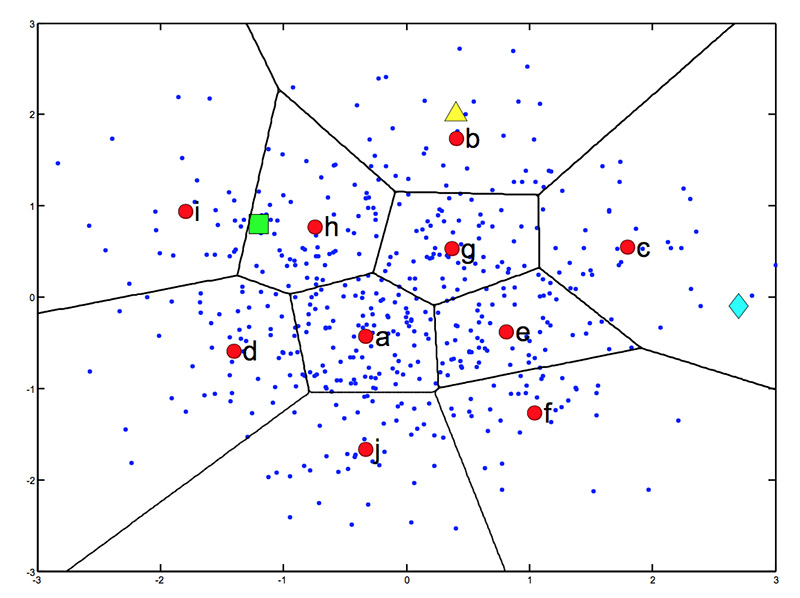
\includegraphics[width=0.35\textwidth]{images/soft-assignment.jpg}
\end{center}
  \caption{\emph{Codeword uncertainty} and \emph{codeword plausibility}}
\label{fig:softAssignment}
\end{figure}

Figure \ref{fig:softAssignment} illustrates both these problems. The small dots represent image features, the labeled red circles are the visual words. The yellow triangle represents a data sample that is well suited to the hard assignment approach. The difficulty with codeword uncertainty is shown by the square, and the problem of codeword plausibility is illustrated by the diamond.

\emph{Soft assignment} coding is proposed to alleviate those drawbacks by assigning a local feature to all visual words. The coding coefficient represents the membership of a local feature to different visual words.

\paragraph{Kernel Codebook}

In Kernel Codebook approach we apply techniques from kernel density estimation to allow a degree of ambiguity in assigning codewords to image features. 

For each word $\omega$ in the vocabulary we evaluate
$$KCB(\omega) = \frac{1}{n} \sum_{i = 1}^{n} K_{\sigma}(D(\omega, r_i))$$
where $n$ is the number of regions, $r_i$ is the image region $i$ and $K_{\sigma}$ is the kernel function defined as
$$K_{\sigma} (x) = \frac{1}{\sqrt{2\pi} \sigma} e^{- \frac{1}{2} \frac{x^2}{\sigma^2}}$$



\section{Image classification}

After assigning each images with a BoF we can proceed to the classification step. For that purpose we evaluated the performance of two type of classifier: \emph{Nearest Neighbor} (NN) and \emph{Support Vector Machine} (SVM).

\paragraph{Nearest Neighbour}

Nearest Neighbours classifies an image in base of the nearest train example. Those classifiers differentiate each other for distance measure used. In this case only Euclidean distance (L2) and $\chi^2$ distance are been used.

\paragraph{Support Vector Machine}

\emph{Support Vector Machines} classifies an image identifying separation surface on feature space. Those surface are evaluated using different kernel functions. The kernels used in our experiments are:
\begin{itemize}
\item \emph{Linear kernel}
\begin{equation}
K(x, z) = <x, z>
\end{equation}
\item \emph{Histogram Intersection kernel}
\begin{equation}
K(x, z) = \sum_{i = 1}^{n} \min (x_i, z_i)
\end{equation}
\item \emph{$\chi^2$ kernel}
\begin{equation}
K(x, z) = \exp (-\gamma \sum_{i = 1}^{n} \frac{(x_i - z_i)^2}{x_i + z_i})
\end{equation}
\item \emph{RBF kernel}
\begin{equation}
K(x, z) = \exp (- \gamma ||x_i - z_i||)
\end{equation}
\end{itemize}
SVM classifier depends on some parameters: C and $\gamma$ values are obtained with 5-fold crossvalidation.

\section{Experimental results}

For our experiments we use a subset of 15 categories of the \emph{Caltech-101} dataset, about 2537 images split between 15 distinct object categories (faces, watches, elephants, motorbikes, etc.)\footnote{\emph{Caltech-101} has been created at the \emph{California Institute of Technology} - http://www.vision.caltech.edu/Image\_Datasets/Caltech101/}. Image descriptors are precomputed over the whole dataset and stored on separate files.. All tests were performed on a Mac OSX Notebook with an Intel Core i5, 8GB (running at 2.4 GHz).

Tests have been made on varying of these parameters: train set size, vocabulary size and SIFT descriptor type (\emph{dense, sparse, multi-scale}). Finally, a comparison between \emph{hard} and \emph{soft assignment} is presented. Test set size is always set to 30 (30 images from each category).

To obtain reliable results, we repeat the experimental processes 10 times, than the mean average accuracy is evaluated.

In Table \ref{tab:trainsetsize} the classification accuracy on varying training set size (the number shown represent how many images are taken from each category) are shown. As we can see in Table \ref{tab:trainsetsize} the larger the training set size the better the accuracy obtained (with fixed vocabulary size) due the greater number of examples used to create the model.

\begin{table}[h]
\begin{center}
\begin{tabular}{|l|c|c|c|}
\hline
Classifier & 10 & 30 & 50\\
\hline\hline
NN $L_2$ & 38,44 & 53,33 & 52,06\\
NN $\chi^2$ & 59,67 & 67,33 & 67,74\\
SVM Linear & 57,56 & 72,44 & 76,58\\
SVM IK & 72,44 & 79,33 & 83,53\\
SVM $\chi^2$ & 72,44 & 79,56 & 83,27\\
SVM RBF & 57,56 & 71,78 & 72,31 \\
\hline
\end{tabular}
\end{center}
\label{tab:trainsetsize}
\caption{Classification accuracy (\%) on varying training set size}
\end{table}

In Figure \ref{fig:vocabulary} it is shown the classification accuracy variation on growing the vocabulary size. All tests have been made fixing training set size to 30 and using \emph{dense SIFT}. Generally the greater the number of codewords used the greater the accuracy obtained. We attribute this performance boost to the ability of the vocabulary to be more expressive, leading to a more discriminant representation of each image.

\begin{figure}[h]
\begin{center}
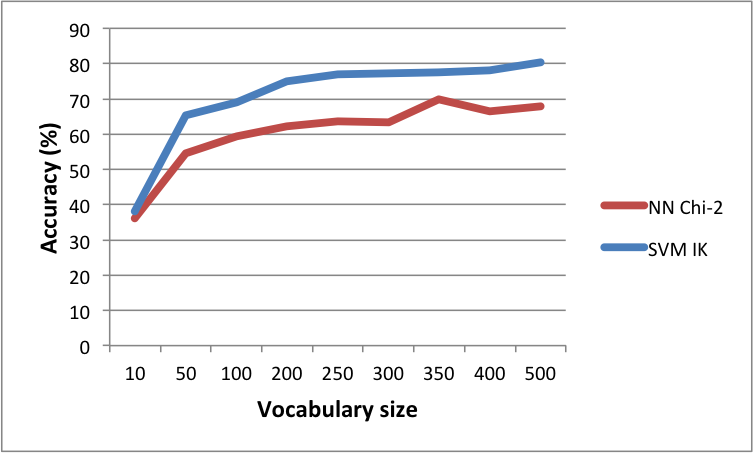
\includegraphics[width=0.45\textwidth]{images/vocabulary.png}
\end{center}
  \caption{Classification accuracy (\%) on growing vocabulary size}
\label{fig:vocabulary}
\end{figure}

In Table \ref{tab:sifttype} it is shown the classification accuracy variation on varying of local features extractor for SIFT descriptor. It is highlighted that dense SIFT reached better accuracy than sparse SIFT due to the greater number of key-points extracted from each images and the spatial homogeneity of key-points distribution. Even better performance is obtained by multi-scale sampling of dense SIFT. 

\begin{table}[h]
\begin{center}
\begin{tabular}{|l|c|c|c|}
\hline
Classifier & \emph{sSIFT} & \emph{dSIFT} & \emph{msdSIFT}\\
\hline\hline
NN $L_2$ & 44 & 49,78 & 52,22\\
NN $\chi^2$ & 57,78 & 68,89 & 68,67\\
SVM Linear & 69,33 & 73,33 & 74,22\\
SVM IK & 77,56 & 81,56 & 81,78\\
SVM $\chi^2$ & 78 & 80 & 82\\
SVM RBF & 71,56 & 71,78 & 71,89 \\
\hline
\end{tabular}
\end{center}
\label{tab:sifttype}
\caption{Classification accuracy (\%) on varying SIFT type}
\end{table}

In Figure \ref{fig:soft} a comparison between hard and soft assignment performance is presented. In the results the kernel codebook method has excluded due its worst results\cite{Gemert:2008:KCS:1478172.1478227}.

The results show that localized codeword uncertainty outperforms both hard assignment and codeword uncertainty. The $k$ value for localized codeword uncertainty has been set to 5. The kernel size obtained by cross-validation for soft assignment is typically 45. As evidenced by Figure \ref{soft}, the \emph{early cut- off} strategy can improve the classification performance of soft-assignment coding.

\begin{figure}[h]
\begin{center}
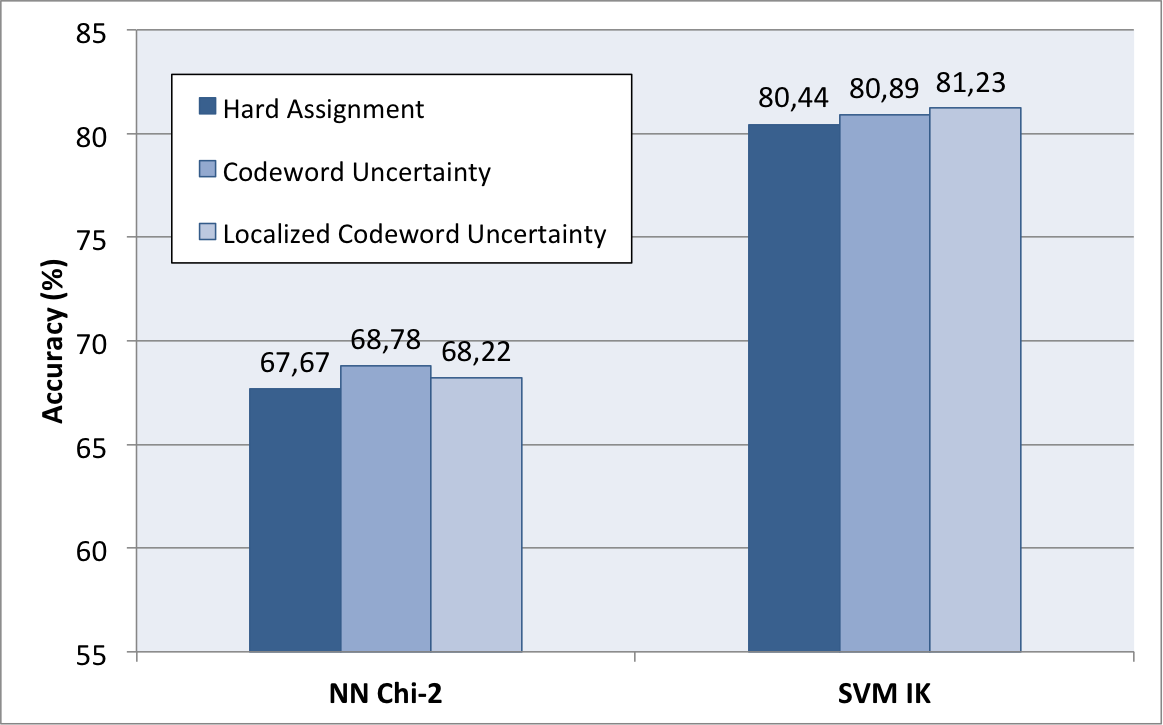
\includegraphics[width=0.45\textwidth]{images/soft-comparison.png}
\end{center}
  \caption{Comparison between hard and soft assignment}
\label{fig:soft}
\end{figure}


\section{Conclusions}

In this paper, we have analysed the performance of two classifiers, \emph{Nearest Neighbor} and \emph{Suppor Vector Machine}, with varying distance functions and kernel functions, using the \emph{Bag of Words} model. 

The experiments taken on the dataset, lead to the conclusion that there are many parameters that can influence the performance of a classifier.
The greater the dimension of the training set, the better the classification accuracy, because more examples lead to a more accurate abstraction of the data model; having more codewords improves the performance due to the fact that a larger vocabulary means a more expressive vocabulary and so a histogram more capable of discriminating between images (however, the accuracy boost of a larger vocabulary eventually saturates); the choice of sparse or dense local features, on which the SIFT descriptors are computed, can also influence the classification accuracy, as shown in Table 2.

Finally, we have analysed how different features quantization can influence the performance of a classifier, in particular the difference between \emph{hard-assignment} and \emph{soft-assignment}, as this was our main focus in this paper.
We have found that by allowing a degree of ambiguity in features quantization, \emph{soft-assignment} is able to improve the classification accuracy of \emph{hard-assignment}. Improvement over the \emph{soft-assignment} can be obtain using the \emph{localized soft-assignment} by taking into account only the k-nearest codewords and in this way removing some noise in the features quantization.

\end{document}
